\documentclass[parskip=full]{scrartcl}
\usepackage[T1]{fontenc}    % avoid garbled Unicode text in pdf
\usepackage[utf8]{inputenc} % use utf8 file encoding for TeX sources
\usepackage[german]{babel}  % german hyphenation, quotes, etc
\usepackage{hyperref}       % detailed hyperlink/pdf configuration
\hypersetup{                % ‘texdoc hyperref‘ for options
pdftitle={PSE: Entwicklung eines relationalen Debuggers - Pflichtenheft},%
,%
}
\usepackage{graphicx}       % provides commands for including figures
\usepackage{csquotes}       % provides \enquote{} macro for "quotes"
\usepackage[nonumberlist]{glossaries}     % provides glossary commands
\usepackage{enumitem}

\makenoidxglossaries


\title{PSE:\\ Entwicklung eines relationalen Debuggers\\ Pflichtenheft}
\author{
	Benedikt Wagner\\
	\texttt{udpto@student.kit.edu}
	\and Chiara Staudenmaier\\
	\texttt{uzhtd@student.kit.edu}
	\and Etienne Brunner\\
	\texttt{urmlp@student.kit.edu}
	\and Joana Plewnia\\
	\texttt{uhfpm@student.kit.edu} 
	\and Pascal Zwick\\
	\texttt{uyqpk@student.kit.edu}
	\and Ulla Scheler\\
	\texttt{ujuhe@student.kit.edu}
}

\begin{document}

\maketitle
\newpage

\tableofcontents
\newpage

\section{Produktübersicht}
%kurze Übersicht über das Produkt
Das Produkt soll dem Nutzer die Möglichkeit bieten, mehr als ein Programm gleichzeitig zu debuggen und interaktiv zu analysieren. Dabei sollen die Konzepte eines herkömmlichen Debuggers, namentlich Einzelschritte, Breakpoints und Variableninspektion, erhalten bleiben und um zusätzliche Konzepte, die den Umgang mit zwei Programmläufen erleichtern, erweitert werden. Der Fokus liegt hierbei in der Unterstützung des Findens von Zusammenhängen in den vom Nutzer in einer WHILE-Sprache verfassten Programmen.

Zielgruppe wo?

\section{Produkteinsatz}
%Anwendungsbereiche, Zielgruppen, Betriebsbedingungen
..

\section{Produktumgebung}
%Software, Hardware, Orgware, Schnittstellen
..

\section{Produktfuntionen}
	\subsection{Funktionale Anforderungen}
		\subsubsection{Musskriterien}
		..
		\subsubsection{Sollkriterien}
		..
		\subsubsection{Kannkriterien}
		..
		\subsubsection{Abgrenzungskriterien}
		..
	\subsection{Nichtfunktionale Anforderungen}
		\subsubsection{Produktdaten}
			\paragraph{/PD10/. Konfigurationsdateien:}
			Diese Dateien speichern eine Konfiguration des Debuggers.
			Zu diesen gehören die Eingabewerte, Schrittgrößen, Variablen Auswahl, 						Quelltext und Position beider Programme, aber nicht die Ausgabewerte, da diese 			vom Programmcode zur Laufzeit generiert werden.
			Weiter müssen alle Breakpoints gespeichert werden. Dazu zählen sowohl gesetzte 			als auch bedingte Breakpoints. Letzteres benötigt keine Speicherung der Zeile, 			sondern eines Bereiches, zwei Variablen der Programmtexte und einen Operator. 				Dies gilt auch für die Watch-Expressions mit Ausnahme eines Bereiches.
			\paragraph{/PD20/ Sprachdateien:}
			Diese Datei speichert die Übersetzung der gesamten Benutzeroberfläche.
			Dazu gehören die Texte auf GUI-Elementen und Tooltips.
			\paragraph{/PD30/ Einstellungsdatei:}
			Diese Datei speichert die zuletzt ausgewählte Sprache und die URL der 						Konfigurationsdatei, welche zur zuletzt verwendeten Konfiguration passt.
		\subsubsection{Produktleistungen}
		..
		\subsubsection{Weitere nichtfunktionale Anforderungen}
		..

\section{Qualitätsanforderungen}
..

\newpage
\section{Anwendungsfälle und Szenarien}
\begin{figure}[h] 
  \centering
     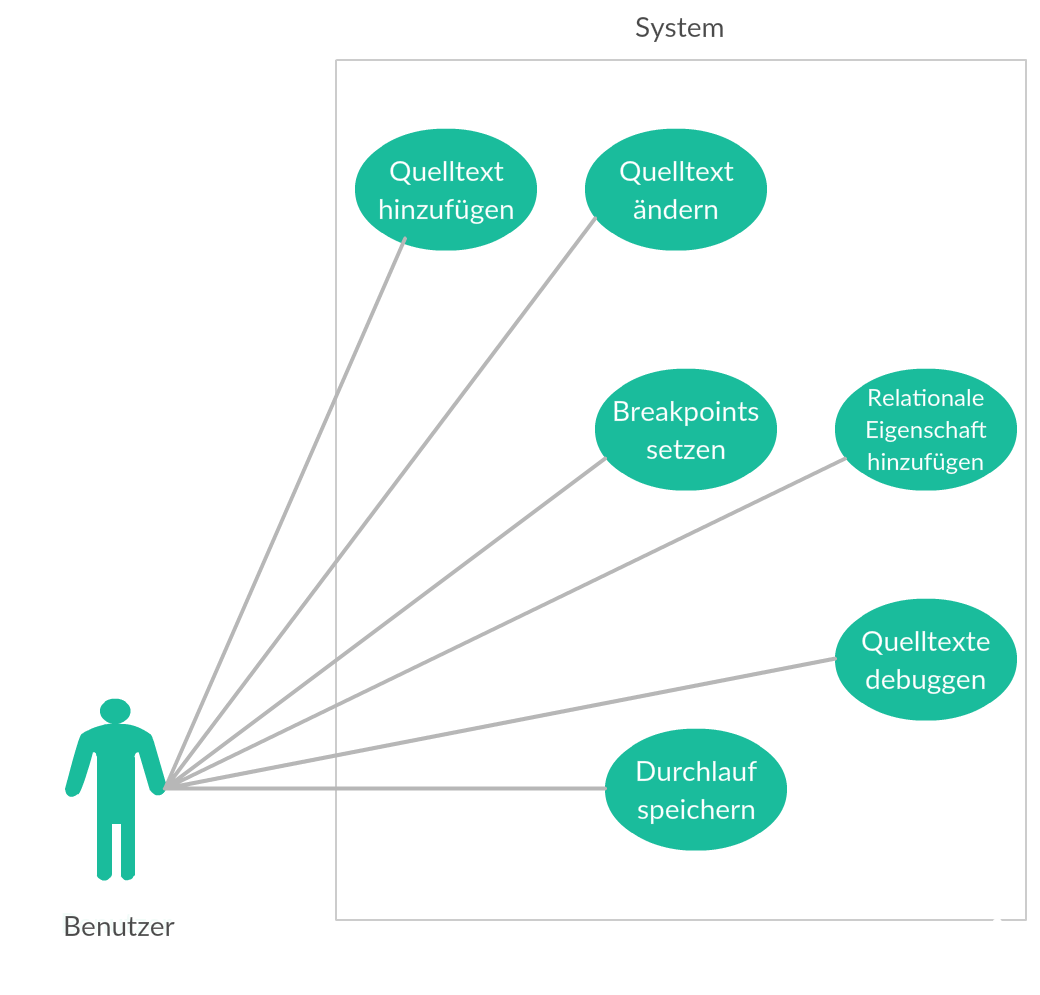
\includegraphics[width=0.7\textwidth]{Anwendungsfalldiagramm}
  \caption{Anwendungsfalldiagramm}
  \label{fig:Bild1}
\end{figure}

\section{Globale Testfälle}
..

\newpage
\section{Systemmodelle}
%Architektur, Verhalten, usw
\begin{figure}[h] 
  \centering
     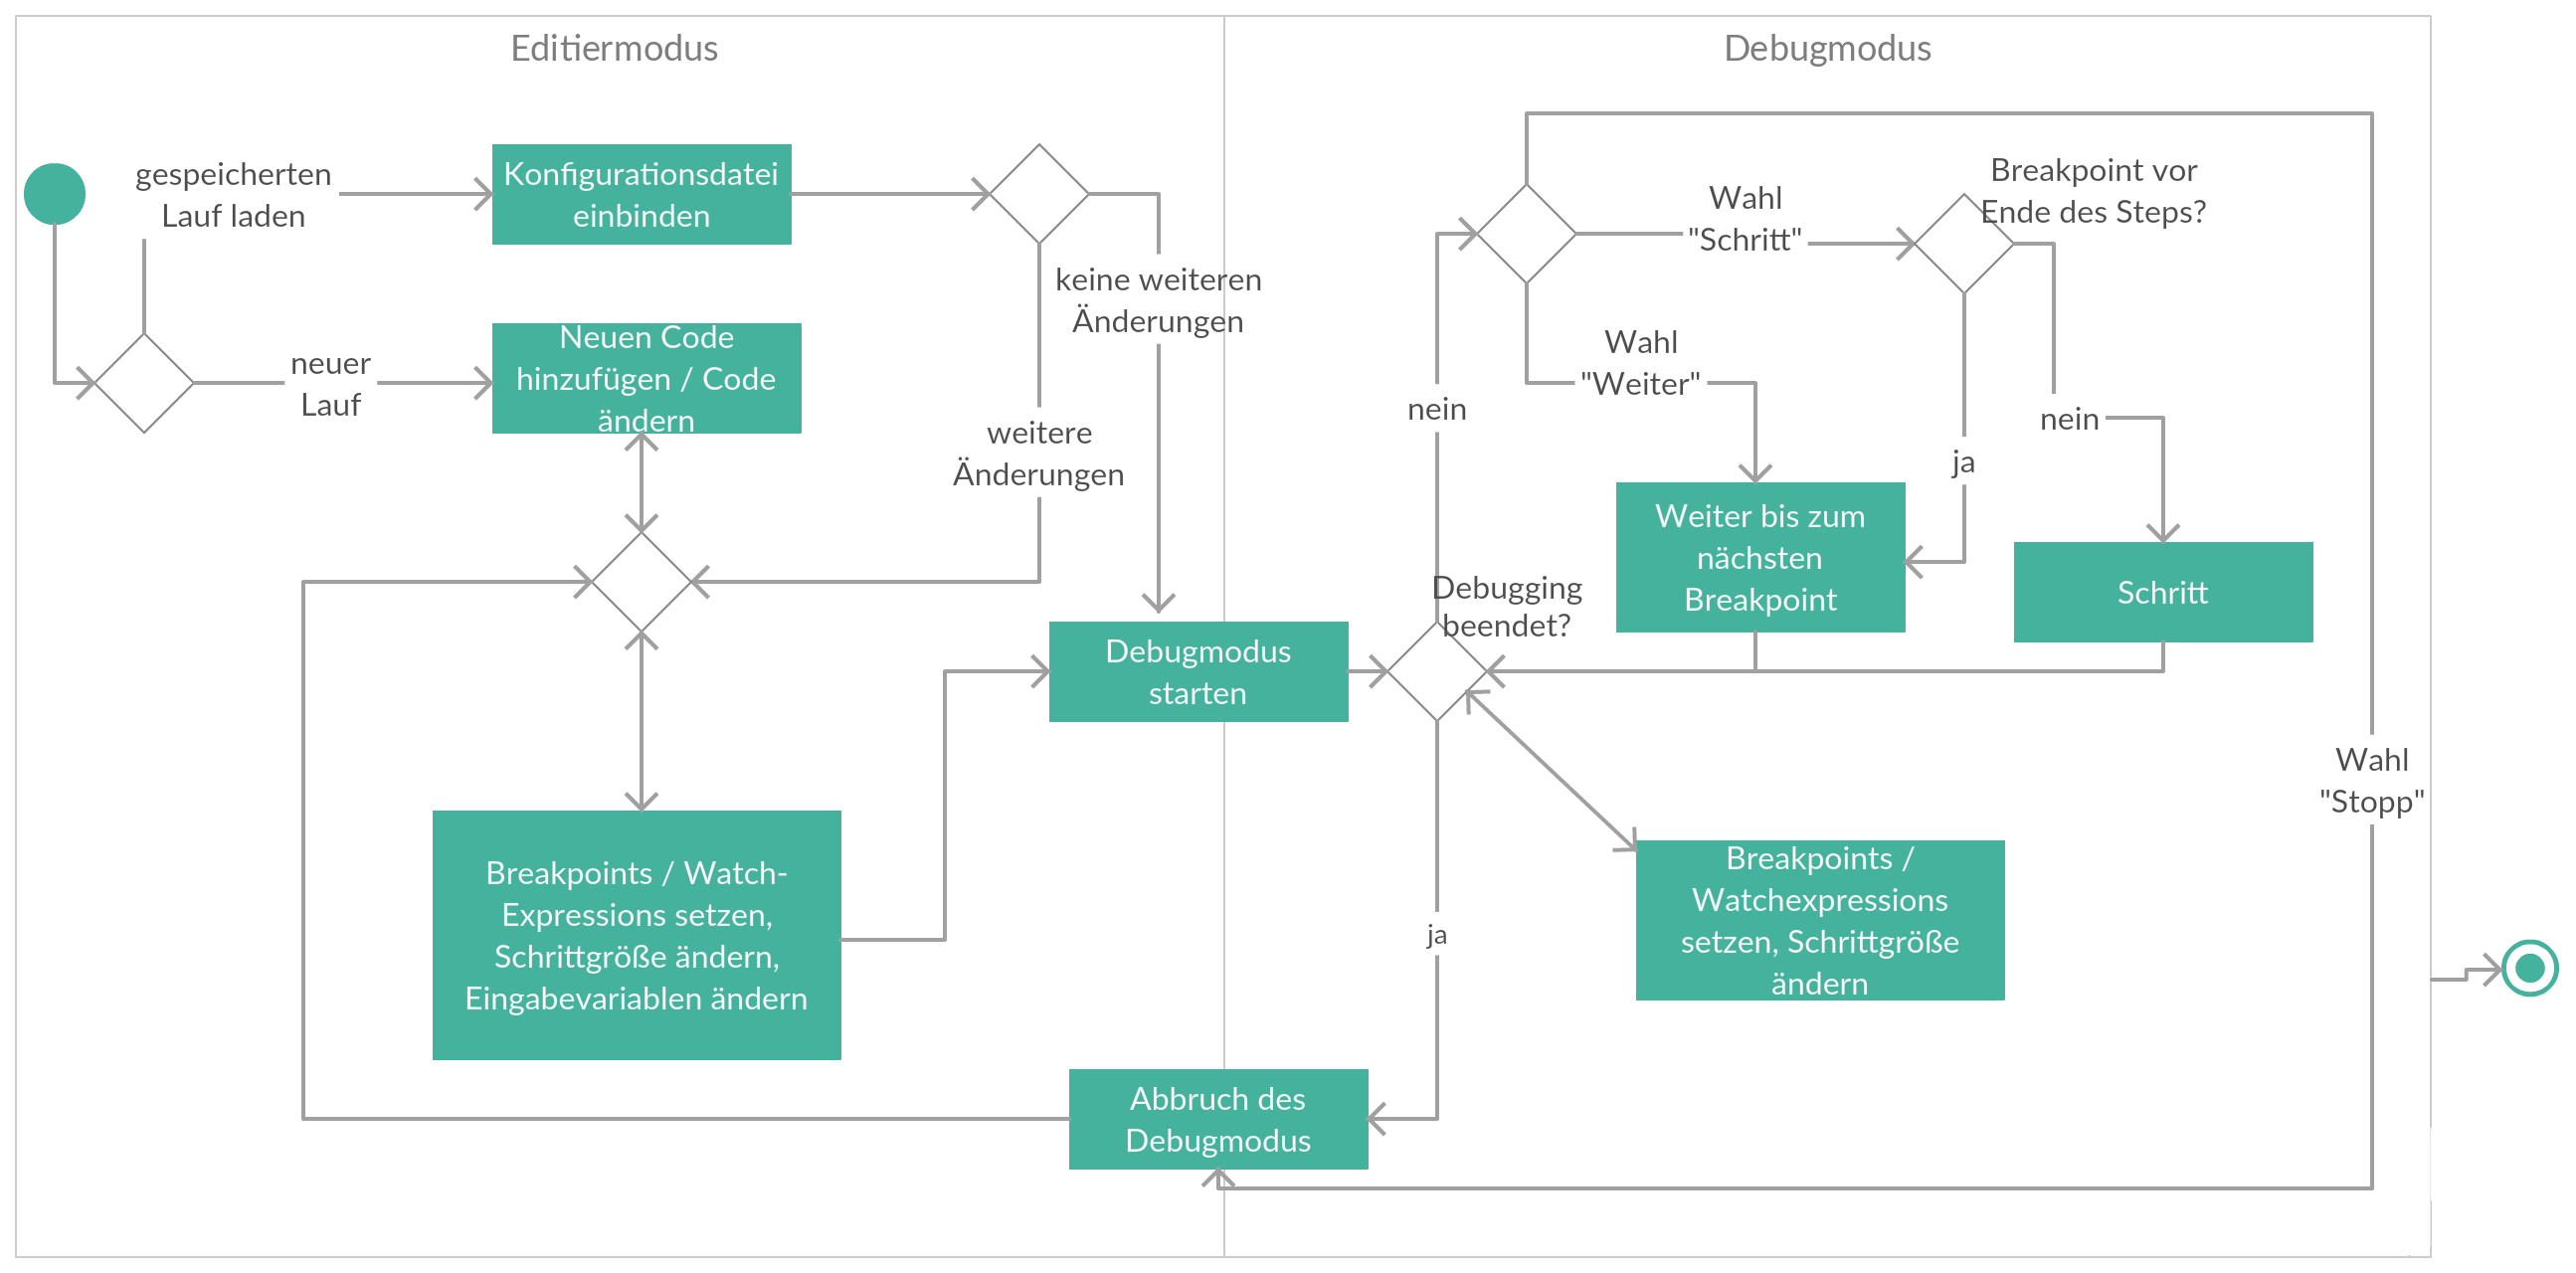
\includegraphics[width=0.9\textwidth]{Aktivitaetsdiagramm}
  \caption{Aktivitätsdiagramm}
  \label{fig:Bild1}
\end{figure}

\newpage
\section{Benutzungsoberfläche}
%Gui-Skizzen, Erklärungen der Menüs, usw
\begin{figure}[!ht] 
    \vspace{-20pt}
    \centering
       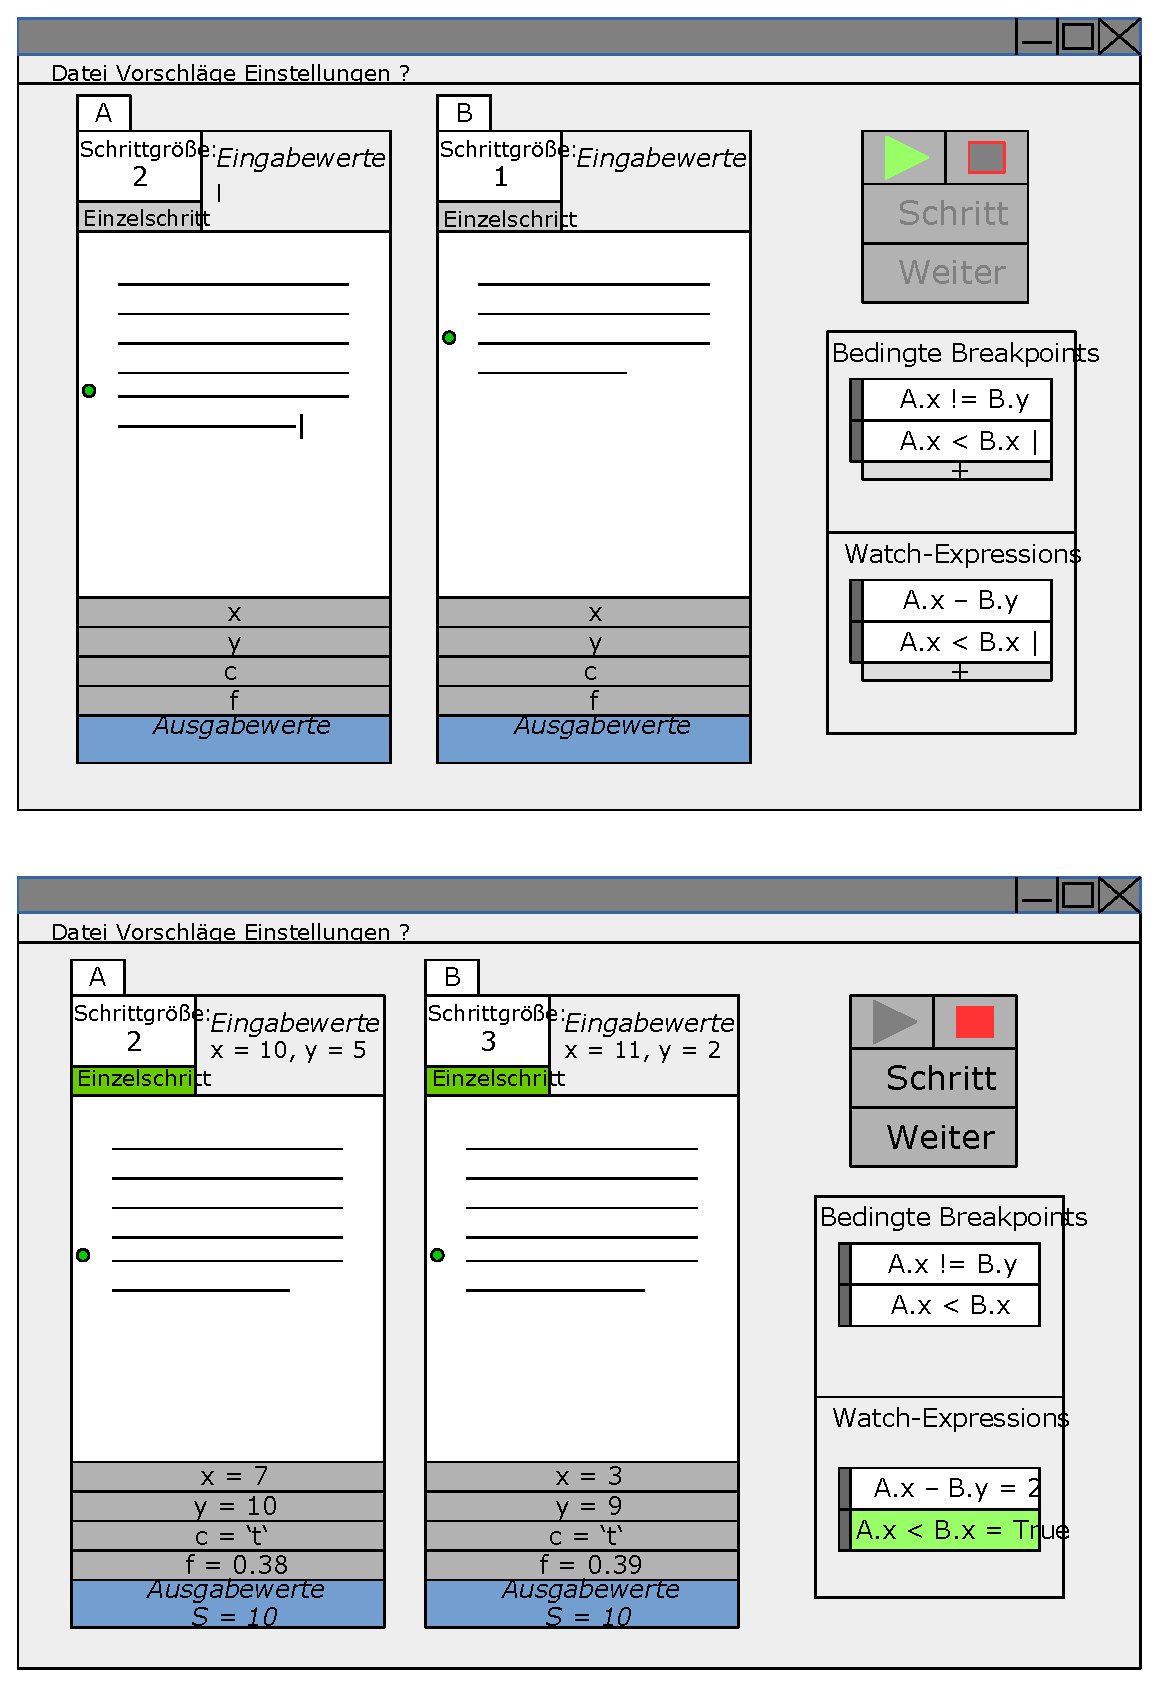
\includegraphics[width=0.9\textwidth]{skizzeFull}
       \caption{
         Benutzeroberfläche von --Programmname-- im Editiermodus (oben) und im Debugmodus
         (unten)
       }
    \label{fig:Bild1}
\end{figure}

    \subsection{Beschreibung}
        Befindet sich --Programmname-- im Editiermodus können die Eingabequelltexte über die 
        Eingabefenster bearbeitet werden.
        Durch Verändern des Textes im Bereich \enquote{Eingabewerte} können Werte der Eingangsvariablen
        spezifiziert, gelöscht und verändert werden. 
        Bedingte Haltepunkte und Watch-Expressions können durch Betätigung der jeweiligen 
        \enquote{+}-Schaltflächen hinzugefügt werden.
        Die Schaltflächen \enquote{Schritt} und \enquote{Weiter}, sowie \enquote{Einzelschritt} können nicht betätigt
        werden. Betätigung der Schaltfläche mit dem grünen Pfeil verursacht den Übergang von
        --Programmname-- in den Debugmodus.
        
        Befindet sich --Programmname-- im Debugmodus, können die Eingabequelltexte nicht
        über die Eingabefenster bearbeitet werden. Die \enquote{+}-Schaltflächen für bedingte Haltepunkte
        und Watch-Expressions können nicht betätigt werden.
        Die Schaltflächen \enquote{Schritt}, \enquote{Weiter} und \enquote{Einzelschritt} können betätigt werden.
        Betätigung der Schaltfläche mit dem roten Viereck verursacht den Übergang von --Programmname-- in den Editiermodus.
        
        
\section{Zeit- und Ressourcenplanung}
..

\section{Ergänzungen}
..

\section{Glossar}




\end{document}
\grid
